%% \chapter[htoc-titlei][hhead-titlei]{htitlei}
%% -----------------------------------------------------------------------------
\chapter[Theorteical Background][Theorectical Background]{Theoretical Background}

The Standard Model of particle physics is an extradinarly successful
description of the fundamental constituents of matter and their interactions.
Experiments over the past 50 years have verified the extremely precise
prediction of the SM; this success has culminated most recently in the
discovery of the Higgs Boson.  This chapter provides a brief introduction to
the structure of the SM and how scientists are able to test it using hadron
collider but focuses primarily on the physics of the Higgs boson and its decays
to top quarks.  Particular attention is given to the importance of a
measurement of the rate at which Higgs Bosons are produced in association of
top quarks in the context of our theoretical understanding of the SM. 


\section{The Standard Model}

The Standard Model (SM) is an example of a quantum field theory that describes
the interactions of all of the known fundamental particles (with the exception
    of the gravitational interaction). It was developed over the course of the
course of many years as the result of both theoretical and experimental
discoveries. Particles are understood to be excitations of the more fundamental
object of the theory, the fiel The dynamics and interactions of the fields are
derived from the Standard Model Lagrangian, which is constructed to be
symmetric under local gauge transformations of the group $SU(3) \times SU(2)
  \times U(1)$. $SU(3)$ is the gauge group for the color, $SU(2)$ is the gauge
  group for weak iso spin, and $U(1)$ is the group for weak hypercharge. 

Gauging the symmetries demands the introduction of 8 massless gluons, or the
boson (full integer spin) carriers of the strong force from the generators
$SU(3)$ symmetry, and the 4 massless electroweak bosons, carriers for the weak
and electronmagnetic forces from the 3 generators of the $SU(2)$ and 1
generator of the $U(1)$ group. The gauge symmetry also allows the theory to be
renormalizable, meaning that unwanted infinities can be absorded into
observables from theory in a way that allows the theory to be able to predict
phyiscs at multiple energy scales.  Singlets of the $SU(3)$ group are fermions
(half-integer spin particles) called leptons (electron, muon, tau, and
    associated neutrinos) and do not interact with the strong, where as
doublets of the $SU(3)$ group are called quarks (up, down, strange, charm, top,
    bottom) and do interact with the strong force. The SM is a chiral theory:
the weak force violates parity, as it only couples to left-chiral particles or
right-chiral antiparticles. This in a sense suggests that right-chiral and
left-chiral fermions are different particles coming different fields, which are
different representations of the weak-isopsin group.

So far, 3 separate generations of both quarks and leptons have been discovered,
   differing only by mass. The reason for this 3-fold replication is not known.
   The heaviest of which is the top quark, discovered at the Tevatron in 1996.
   The gluon and the 4 electroweak bosons have also been found ($W^+$, $W^-$,
       $Z^0$, and $\gamma$). 


\section{Electoweak Symmetry Breaking and the Higgs}

Despite the simple structure of theory, the discovery of massive fundamental
particles creates two sets of problems both related to $SU(2) \times U(1)$
gauge invaraince. First, the force-carrying bosons must enter the theory
without mass in order for gauge symmetry to be preserved. Second, adding
fermion masses to theory in an ad-hoc way allows the right-chiral and
left-chiral fermions to mix. Since they possesses different quantum numbers, as
different representations of the weak-isospin group, this too breaks gauge
invariance. 

To solve these problems, spontaneousy electro-weak symmetry breaking (EWSB) is
introduced via the Brout-Englert-Higgs(BEH) mechanism. Massive scalar fields,
in an electro-weak doublets, are introduced into the theory with 4
degrees of freedom and a specific potential, which includes
self-interaction provides the mechanism for spontaneous symmetry
breaking. The fermion fields interact with Higgs field with via a
Yukawa coupling term, which unites the left and right chiral fields
of a single particle type.  The minimum of the potential does not
occur when the expectation of the field is zero. The field
eventually falls to a state, where it aquires a vacuum-expectation
value. However, a non-zero field must therefore point in a
particular direction of weak-isospin space, breaking the symmetry.

The consquences of this spontaneousy symmetry breaking are tremendous. First,
the universe is filled with the Higgs field at its new vaccuum expectation
value. The theory can be expanded around the new mininum and 3 of the
degrees of freedom can be interpreted as the longitundinal polarizations of
the $W^+$, $W^-$, and $Z^0$, while the 4th remains a scalar field, called
the Higgs field. The weak bosons thus aquire a mass and the yukawa
couplings of the scalar field to the fermions now behave like a mass term
at the new mininum. 


\subsection{The Standard Model Parameters}

Although the SM structure can be set by specifiying the gauge groups, EWSB
mechanism, and acknolwedging the 3-fold replication of the fermions,
confronting the SM with experiment requires the measurment of
17\footnote{There are additional parameters from neutrino mass terms and
mixing but it is unclear how to include these into the Standard Model,
since it does not predict right-chiral neutrinos} free parameters, which
are uncontrained from the theory. These free parameters include the fermion
masses, coupling constants, the angles and phase of the mixing between
quarks, constants from the massive neutrino sector, and constants from the
higgs and electroweak sector\footnote{ The electroweak sector includes
parameters like mass of the $W^{\pm}$ and $Z^0$ bosons, the weak mixing
angle,${\mathrm sin^2}\theta_w$, the fermi constant $G_F$, and Higgs
Mass and vacuum-expecation value. These parameters however are not
wholly indepenent. As discussed above, it is only necessary
theoretically to specify the two parameters relevant to the Higgs
potential and the two coupling associated with the gauge groups }.

%arXiv:1209.2716v2%
Experiments have provided a number of measurements over the years of various
parameters of the SM. Although the Higgs Boson particle was only discovered recently,
the integration of the Higgs field into SM mean that the $vev$ could
be constrained prior to discovery from other measurements. The Higgs mass,
however, remained theoretically unconstrained. 
However, it could be inferred in the context of the SM
constainted via its dependence on loop corrections from the top mass
($M_t$) and the W mass ($M_W$). The GFitter collaboration assembles
all relevant electroweak obervable measurements into a statistical
model and then allows certain measurements to float within their
uncertainty to allow for parameter overconstraints among multple
measurements. Figure \ref{figure:theory_scans} shows the fitted constaints on 4 key SM
parameters ($M_H$, $M_W$, $M_t$, ${\mathrm sin^2}\theta_w$) and
actual measuremetns. The addition to the fit of the measured
Higgs mass from the ATLAS and CMS collaborations creates a small
tension, as the other observables prefer the mass to be much
lower ($\sim$ 80 \gevcc). The tension in the combined
electroweak fit (including the Higgs) is not statsitcally
significant with a $p$-value of 0.07.  


\begin{figure}[!t]
\centering 
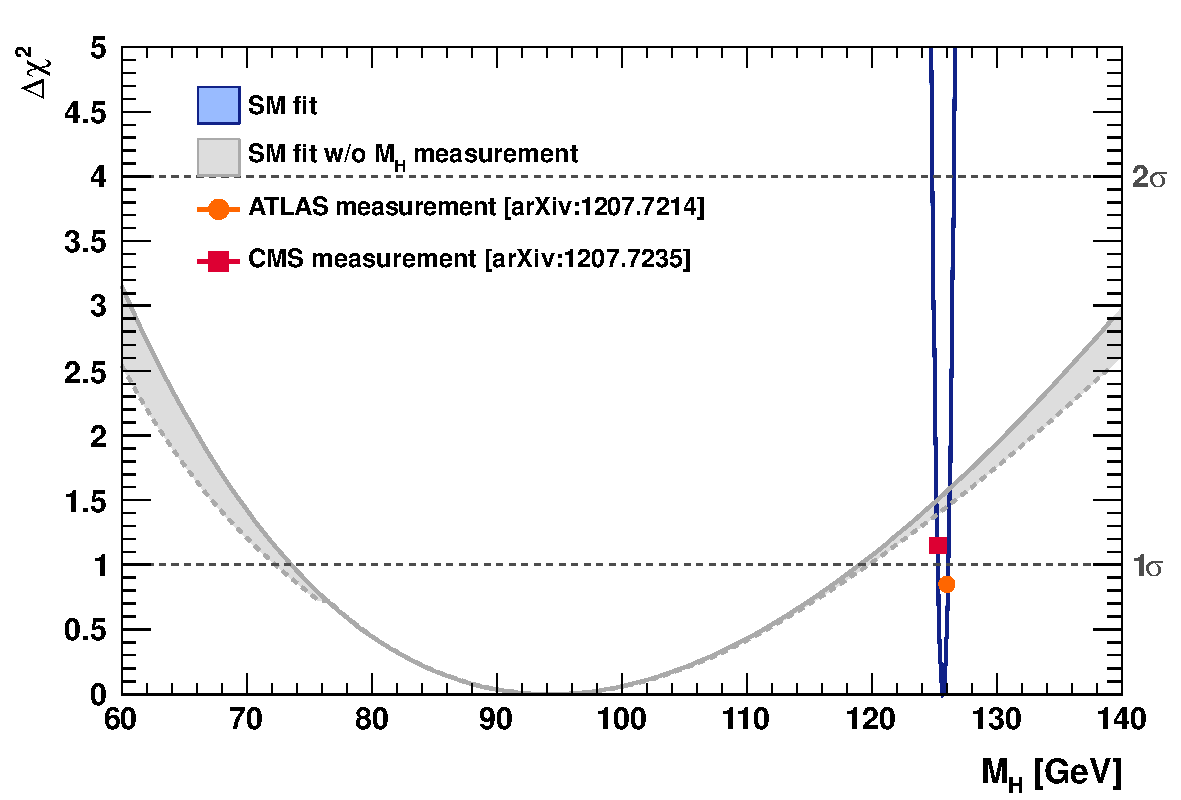
\includegraphics[width=0.35\textwidth]{figs/HiggsScan.pdf}
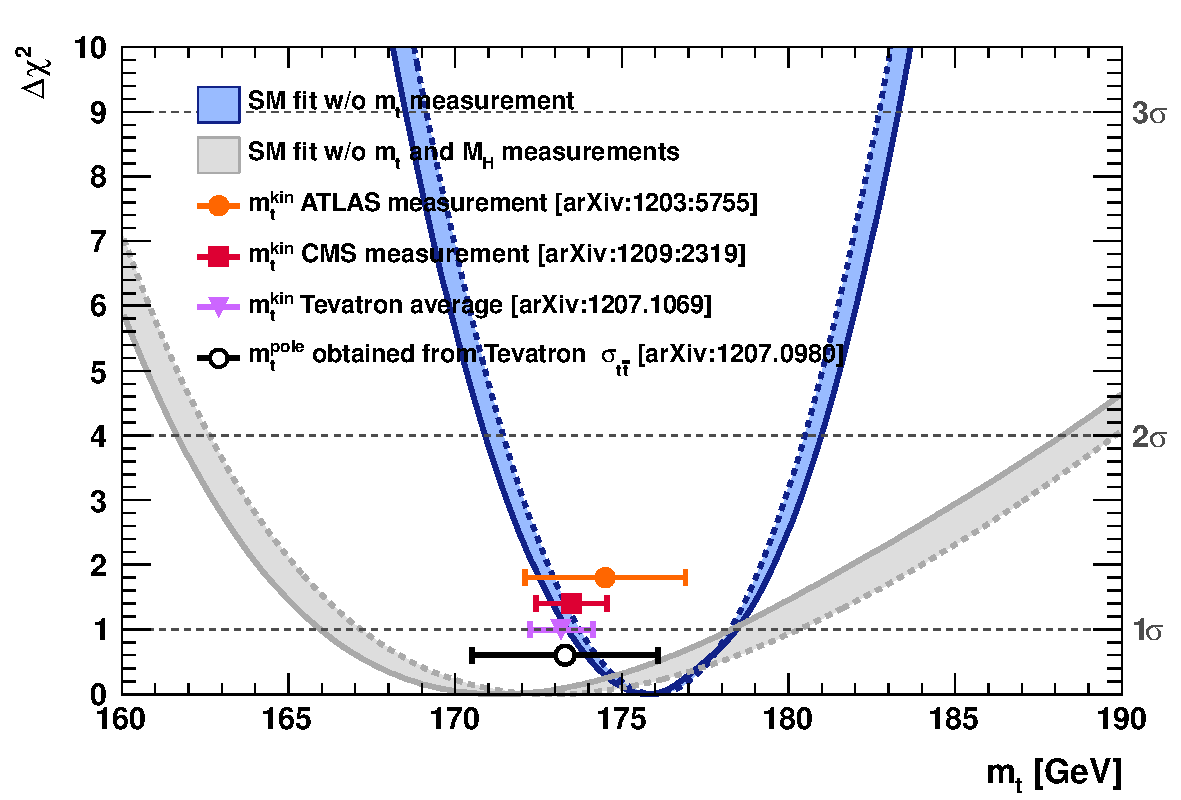
\includegraphics[width=0.35\textwidth]{figs/TopScan.pdf}
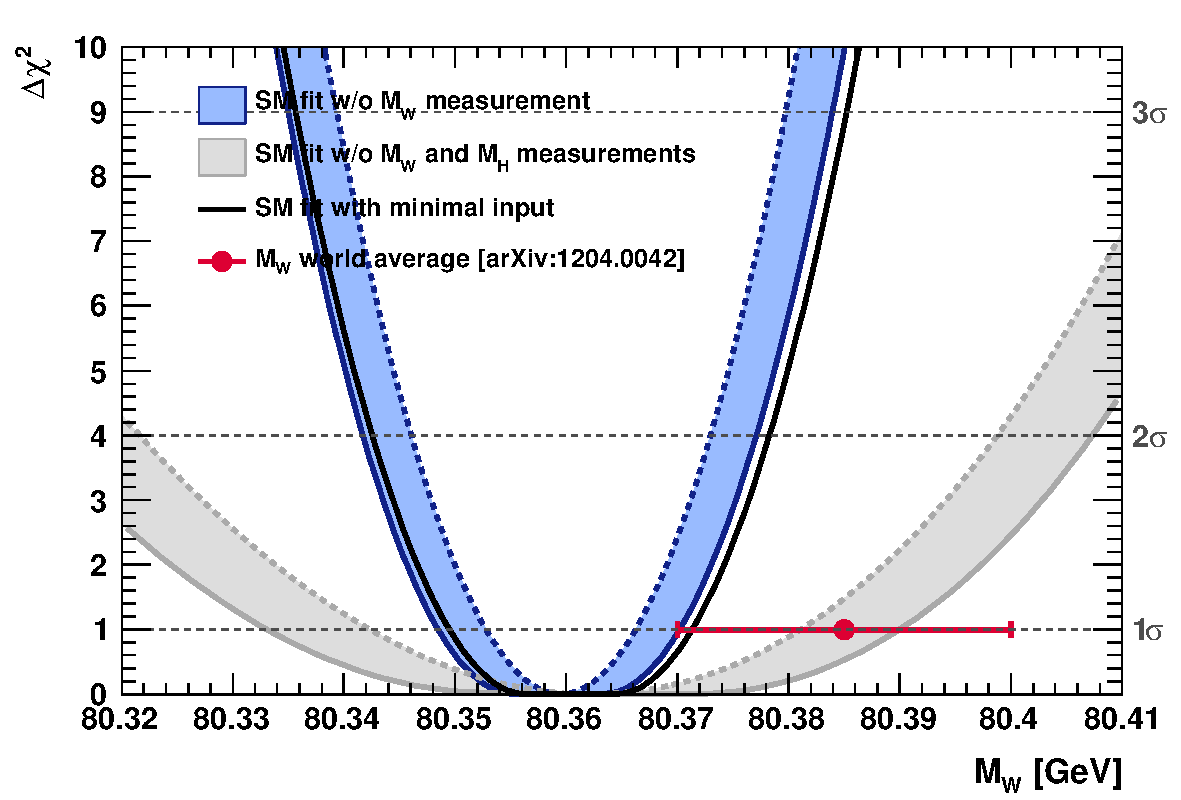
\includegraphics[width=0.35\textwidth]{figs/WMassScan.pdf}
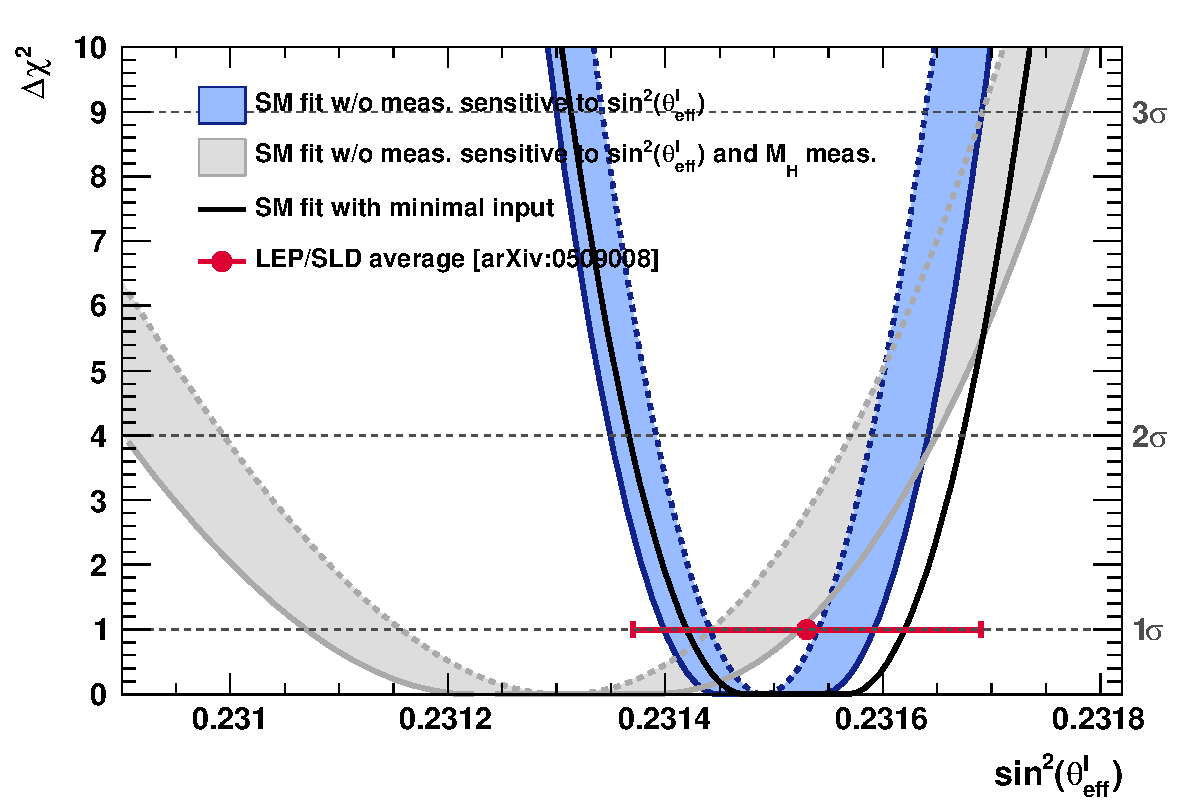
\includegraphics[width=0.35\textwidth]{figs/Sin2ThetaScan.pdf}
\caption{
$\chi^2$ as a function of the Higgs mass (topleft), the top quark mass (top
    right), the $W$ boson mass (bottom left) and the effective weak mixing
  angle (bottom right) for the combined SM fit from the GFitter group.  The
  data points placed along $\chi^2=1$ represent direct measurements of the
  respective observable and their $\pm 1\sigma$ uncertainties.  The grey (blue)
  bands show the results when excluding (including) the new $M_H$ measurements
  from (in) the fits. } \label{figure:theory_scans}
\end{figure}


\section{Collider Physics and the Higgs} 

Particle physicists accelerate particles to extremely high energies and force
them to interact through collisions. Typically, the particles accelerated are
electrons or protons, since they are stable. Electron-positron collider
machines have a rich history of discovery and measurement in particle physics.
The advantage of electron accelerators is that the colliding element is itself
a fundamental particle. However, due synchotron radiation, curvature of the
beam line becomes problematic for high energy beams.  Hadron colliders,
specifically, proton-proton and proton-anti-proton (like the Large Hadron
    Collider) colliders can be accellerated in rings without large losses
due to synchotron radiation, but the actual colliding objects at high
energies are the constitutent quarks and gluons. This complicates analysis
because the initial state of the system is not clear on a per-collision
basis and there is not conservation of momentum along the beam direction.
Collider physics rely on form-factor descriptions of the colliding hadrons
(usually protons) that describe the fraction of momentum carried by the
hadrons constituent 'partons'.  These are called parton-distribution
functions, seen in Figure \ref{figure:theory_pdf}, and are integrated
through the theoreritical calculations of various collision processes.

%http://arxiv.org/pdf/0901.0002v3.pdf
At the Large Hadron collider, therefore the types of initial states are
quark-quark, quark-gluon, and gluon-gluon. Gluon collisions dominate overall,
  due to the large number of gluons inside the proton seen in the figure.
  Though the relative importance of different initial states changes with the
  energy scale of the collision and the type of final state sought after.  

\begin{figure}[!t]
\centering 
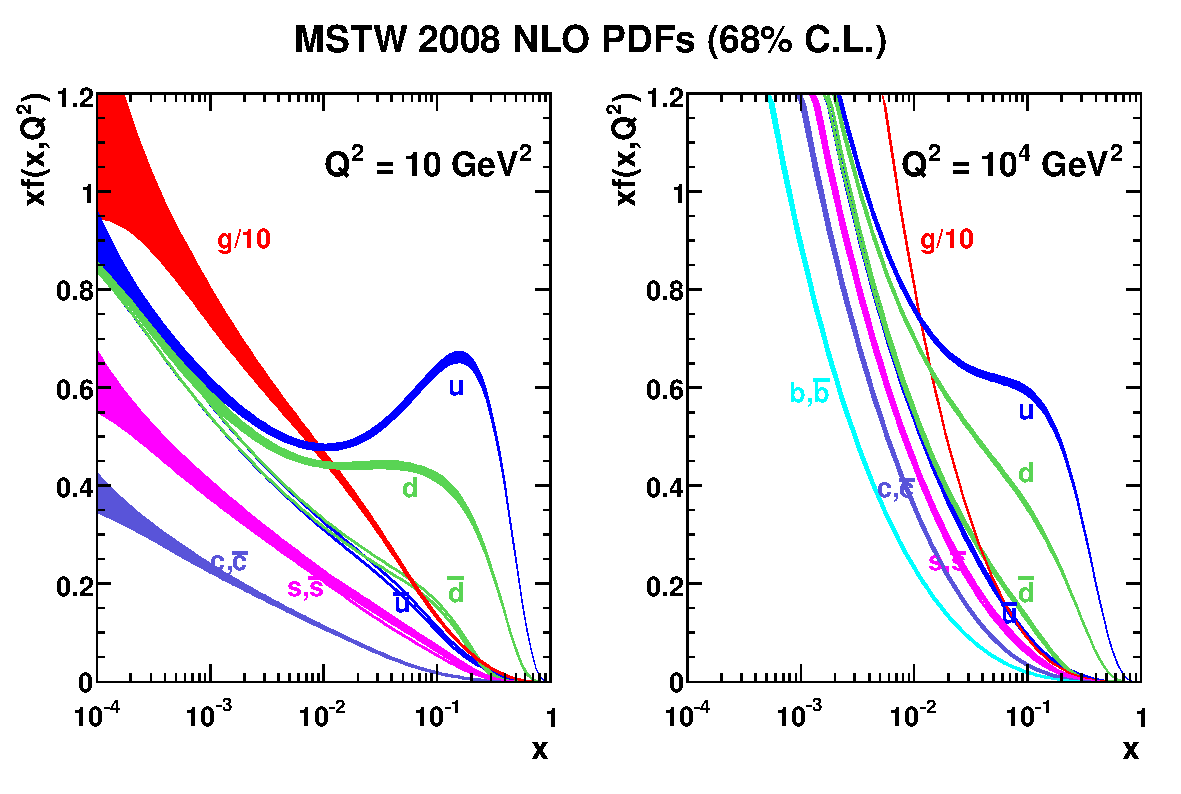
\includegraphics[width=0.8\textwidth]{figs/mstw2008nlo68cl_allpdfs.pdf}
\caption {Proton Parton Distribution Functions (PDFs) form the MSTW Collaboration at $Q^2 = 10$ GeV$^2$ and $Q^2 = 10^4$ GeV$^2$}.
\label{figure:theory_pdf}
\end{figure}

%

%
A prime movitavation for the construction of the Large Hadron Collider was the 
discovery or exclusion of the Higgs boson. LEP and the Tevatron excluded
large swaths of possible Higgs boson masses, especially below 114 \gevcc and
the unitarity of certain diagrams including the $WWWW$ vertex required the 
mass to be below about 1 TeV. 

Despite the ubiquity of Higgs couplings, Higgs boson production at the LHC is a low
rate process. Because it couples to fermions proporitonal to mass and because
the colliding particles must be stable and therefore light, production of the Higgs must occur
through virutal states. 

The Higgs boson can be produced through collision at the Large Hadron Collider via 4 mechanisms: gluon-fusion, 
vector-boson fusion, associated production or higgs strahlung, and production in association with 
top quarks. The diagrams are shown in Figure \ref{theory_higgsdiagrams} and the production cross-sections as a function of Higgs mass for
the 8 TeV LHC proton-proton runinng are shown in Figure \ref{figure:theory_xsec}. The largest production cross-section is via the gluon fusion channel at ~$20$ pb,
which proceeds through a fermuion loop that is dominated by the top quark, because of its large yukawa coupling to the Higgs. Because
the Higgs' couples to every massive particle, it has a rich decay topology also seen in Figure \ref{figure:theory_xsec}, especially for $m_H=100$.
Studies of Higgs properties at hadron colliders offers rich tests of the Standard Model, which is already overconstrained, and ample room
for searches for new physics. These tests specifically can verifiy the link between Yukawa coupling and the particles mass andfurther 
cosntrain details of EWSB by examing Higgs coupling to the weak bosons. 

\begin{figure}[!t]
\centering 
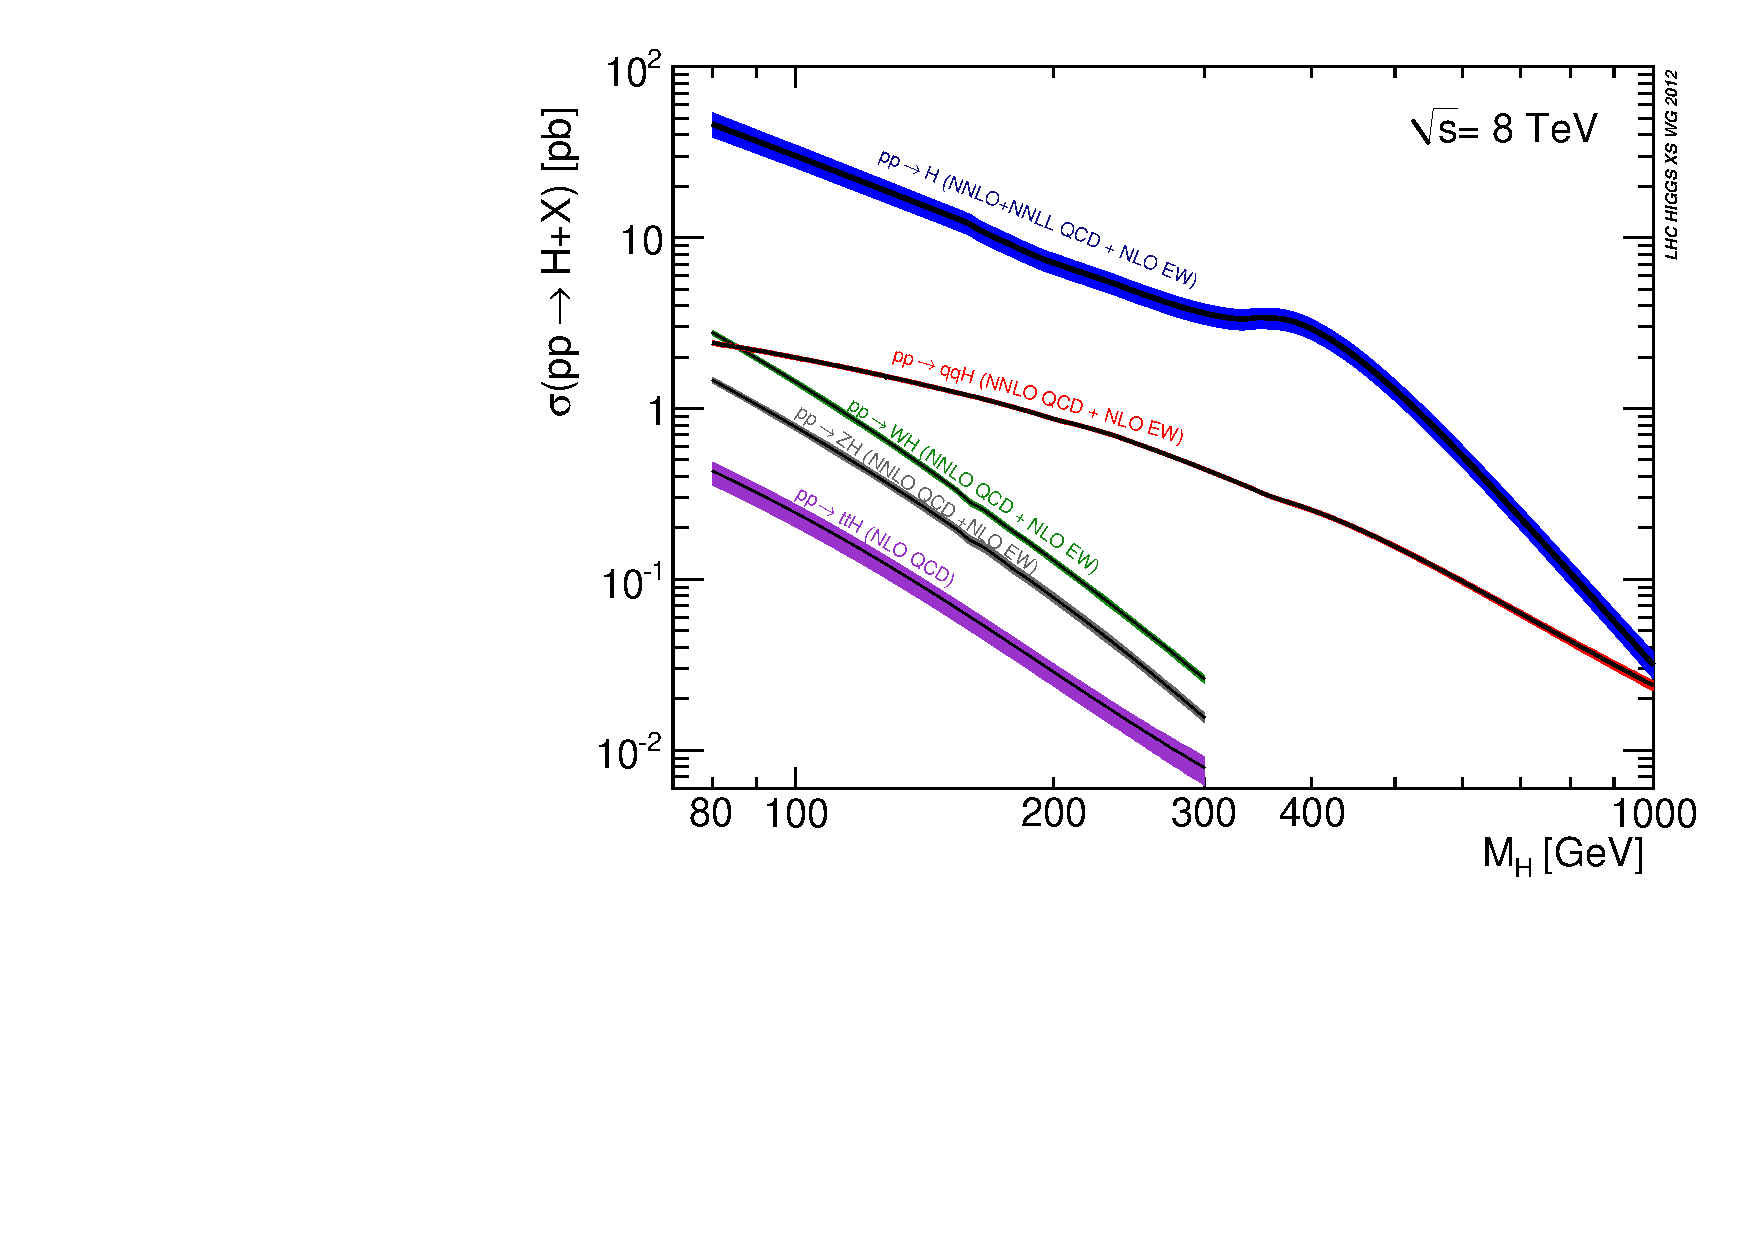
\includegraphics[width=0.52\textwidth]{figs/Higgs_XS_8TeV_lx.pdf}
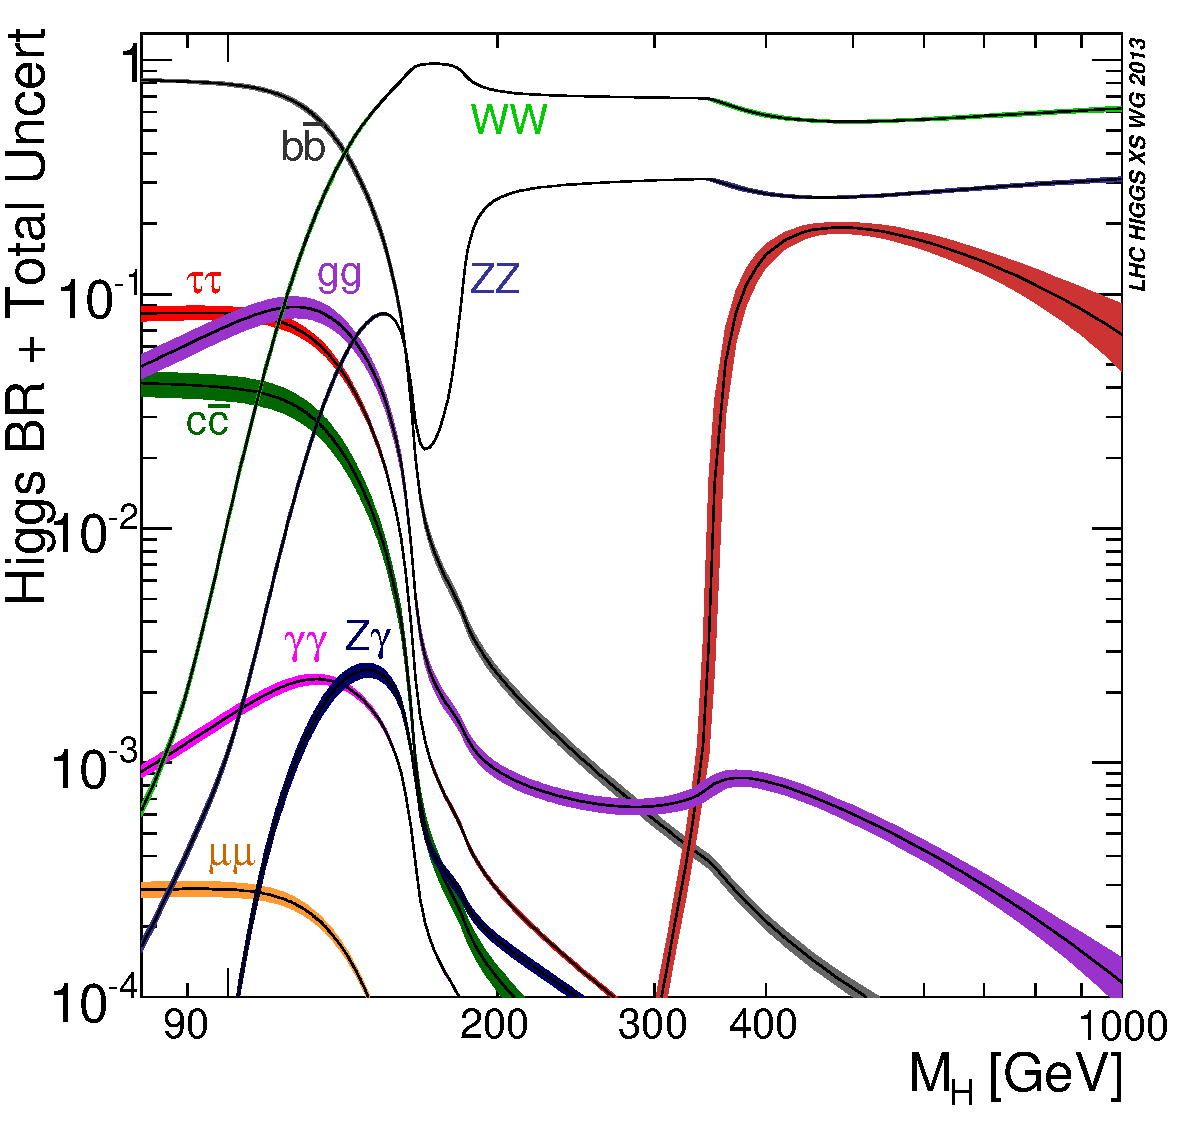
\includegraphics[width=0.42\textwidth]{figs/Higgs_BR.pdf}
\caption {Proton Parton Distribution Functions (PDFs) form the MSTW Collaboration at $Q^2 = 10$ GeV$^2$ and $Q^2 = 10^4$ GeV$^2$}.
\label{figure:theory_xsec}
\end{figure}

\begin{figure}[!t]
\centering 
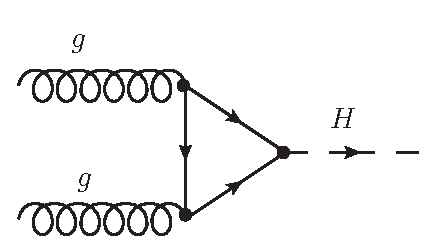
\includegraphics[width=0.35\textwidth]{figs/ggF.pdf}
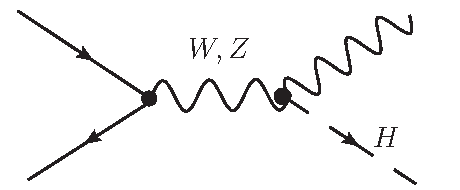
\includegraphics[width=0.35\textwidth]{figs/vh.pdf}
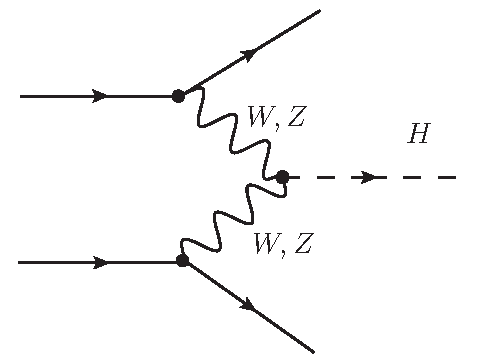
\includegraphics[width=0.35\textwidth]{figs/vbf.pdf}
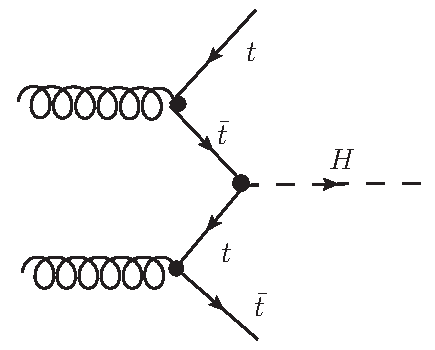
\includegraphics[width=0.35\textwidth]{figs/tth.pdf}
\caption {Proton Parton Distribution Functions (PDFs) form the MSTW Collaboration at $Q^2 = 10$ GeV$^2$ and $Q^2 = 10^4$ GeV$^2$}.
\label{figure:theory_higgsdiagrams}
\end{figure}



\subsection{Higgs Discovery at the LHC}

In 2012 both ATLAS and CMS announced the discovery of a new boson consistent with the Higgs by examining the results of Higgs seaches in a number
of decay channels ($H\rightarrow W^+W^-$,$H\rightarrow Z^0Z^0$, and $H\rightarrow\gamma\gamma$) in the 2011 dataset at $\sqrt{s}=$7 TeV and
part of the 2012 dataset at $\sqrt{s}=8 TeV$. By 2013 and 2014, both experiments have updated and/or finalized their results for the 
full 2011 and 2012 datasets. I will focus on the ATLAS results in the following. These results constrain both the Higgs mass and
spin, as well as a comparison of the coupling strengths of the Higgs to fermions and bosons in various schema. 

%evidence for vbf? vv? vh? already. make this point. -> plots of these parameters




\subsection{Higgs Decays to Top Quarks}

\section{Isseus }
